\chapter{Аналитический раздел}

В данном разделе проводится обзор современных СУБД и анализ их инструментов для управления индексами.

\section{Современные СУБД}

Рассмотрим современные СУБД по таблице \ref{table:list_dbms}.

\begin{table}[h]
\caption{Рейтинг СУБД}\label{table:list_dbms}.
\medskip
\begin{tabular}{|l|p{1.5cm}|p{2cm}|p{7cm}|}
\hline
название & год выпуска & поддержка sql & разработчик\\
\hline
MySQL & 1995 & да & Oracle\\
PostgreSQL & 1995 & да & сообщество\\
MS SQL Server & 1988 & да & Microsoft\\
MongoDB & 2009 & нет & MongoDB\\
SQLite & 2000 & да & Hwaci, сообщество\\
Oracle Database & 1979 & да & Oracle\\
Firebird & 2000 & да & сообщество\\
CouchDB & 2005 & нет & Apache\\
DB2 & 1995 & да & IBM\\
MariaDB & 2009 & да & MariaDB Corporation Ab, MariaDB Foundation, сообщество\\
RavenDB & 2009 & нет & Hibernating Rhinos\\
Redis & 2009 & нет & Redis Labs, сообщество\\
SAP ASE (ex: Sybase) & 1988 & да & SAP AG\\
Percona Server & 2006 & да & Percona\\
\hline
\end{tabular}
\end{table}

Рейтинг СУБД выпускается впервые и сформирован на основе анкетирования (проводилось с августа 2014 по апрель 2016 года) 390 digital-агентств с продакшном и/или клиентским офисом в России: респондентам предлагалось выбрать один или несколько вариантов ответа на вопрос ''Укажите СУБД, которые вы используете при разработке проектов''. \cite{tagline.ru:List_DBMS}

Большинство реляционных СУБД, за исключением MS Access, состоят из двух отдельных компонентов: ''back-end'', где хранятся данные и ''front-end'' — пользовательский интерфейс для взаимодействия с данными. Этот тип конструкции достаточно умный, так как он распараллеливает двухуровневую модель программирования, которая отделяет слой данных от пользовательского интерфейса и позволяет сконцентрировать рынок ПО непосредственно на улучшении своих продуктов. Эта модель открывает двери для третьих сторон, которые создают свои приложения для взаимодействия с различными базами данных. \cite{habrahabr.ru:10_best_tools} 

Данный подход позволяет сторонним разработчикам создавать инструменты для администрирования СУБД. Рассмотрим некоторые СУБД и предлагаемые инструменты для их администрирования, а в частности, индексирования более подробно.

\section{Oracle}

Oracle Database – СУБД, ориентированная на применение в корпоративных сетях распределенной обработки данных (Enterprise Grid), в облачных системах (Cloud Computing), а также для построения корпоративных информационных систем. Она позволяет сократить расходы на информационные технологии благодаря автоматизации управления, использованию недорогих модульных компонентов и кластеризации серверов в целях эффективного использования ресурсов. 

Архитектура СУБД Oracle рассчитана на работу с огромными объемами данных и большим (десятки и сотни тысяч) числом пользователей; она демонстрирует широкие возможности обеспечения высокой готовности, производительности, масштабируемости, информационной безопасности и самоуправляемости. СУБД Oracle может быть развернута на любой платформе, начиная от небольших серверов-лезвий и заканчивая симметричными многопроцессорными компьютерами и мейнфреймами. Уникальная способность СУБД Oracle работать со всеми типами данных, от традиционных таблиц до XML-документов и картографических данных, позволяет рассматривать ее в качестве оптимального выбора для работы с приложениями оперативной обработки транзакций, поддержки принятия решений и управления коллективной работой с информацией.  

\paragraph{Oracle Tuning Pack} – дополнительная опция для управления Oracle Database, наиболее эффективное и легкое в использовании решение, которое полностью автоматизирует процесс настройки приложений. Улучшение производительности SQL достигается с помощью мониторинга выполнения SQL в реальном времени и SQL-советников, интегрированных с Oracle Enterprise Manager Cloud Control 12c, и все это вместе предоставляет всестороннее решение для сложной и требующей много времени задачи по настройке приложений.

\textit{SQL Tuning Advisor} является ответом Oracle на все недостатки и проблемы ручной настройки SQL. Он автоматизирует процесс настройки SQL путем всестороннего исследования всех возможных вариантов настройки SQL-предложения. Анализ и настройка осуществляются с помощью существенно улучшенного оптимизатора запросов, встроенного в ядро базы данных.

\textit{SQL Tuning Advisor} проводит шесть типов анализа:

\begin{enumerate}
\item Анализ статистики: выявление объектов с отсутствующей или устаревшей статистикой, выдача соответствующих рекомендаций по устранению проблемы.
\item SQL-профилирование: Эта возможность, появившаяся в Oracle Database 10g, революционизировала подход к настройке SQL. SQL-профилирование позволяет настраивать SQL-предложения без каких-либо изменений кода приложения.
\item Анализ путей доступа: Во время этого анализа определяются новые индексы, которые могут значительно улучшить производительность запросов.
\item Анализ структуры SQL: Здесь проверяется неявное преобразование типов и даются рекомендации по изменению кода SQL.
\item Степень параллелизма: SQL Tuning Advisor определяет, можно ли улучшить время выполнения с помощью параллельных потоков на определенных этапах выполнения SQL.
\item Альтернативные планы: Во время этого анализа SQL Tuning Advisor находит другие планы выполнения запроса, используя текущие и исторические данные производительности.
\end{enumerate}

Он всесторонне анализирует всю нагрузку и дает рекомендации по созданию новых секций таблицы или индексов, удалению неиспользуемых индексов, созданию новых материализованных представлений и журналов. Определение оптимальной стратегии секционирования или индексирования для конкретной нагрузки является сложным процессом, требующим опыта и времени. SQL Access Advisor учитывает стоимость операций ввода/обновления/удаления в дополнение к запросам и дает соответствующие рекомендации, сопровождаемые количественной мерой ожидаемого выигрыша в производительности, а также скрипты, необходимые для реализации этих рекомендаций. 

Настройка SQL-предложений больше не является прерогативой только специалистов. Oracle встроила эксперта по настройке SQL в ядро базы данных, позволив администраторам баз данных выполнять эту очень важную задачу за доли времени и затрат, необходимых для выполнения той же задачи вручную.

\cite{fors.ru:Oracle-Database}

\subsection{MS SQL Server}

Данный программный продукт представляет собой СУБД реляционного типа, разработанную корпорацией Microsoft. Для манипуляции данными используется специально разработанный язык Transact-SQL. Команды языка для выборки и модификации базы данных построены на основе структурированных запросов.

СУБД является частью длинной цепочки специализированного программного обеспечения, которое корпорация Microsoft создала для разработчиков. А это значит, что все звенья этой цепи (приложения) глубоко интегрированы между собой. То есть их инструментарий легко взаимодействует между собой, что во многом упрощает процесс разработки и написания программного кода. Примером такой взаимосвязи является среда программирования MS Visual Studio. В ее инсталляционный пакет уже входит SQL Server Express Edition. \cite{internet-technologies.ru:SQL-Server}


\paragraph{Database Engine Tuning Advisor}

Помощник Database Engine Tuning Advisor анализирует рабочую нагрузку и выдает рекомендации по физической структуре одной или нескольких баз данных. Анализ содержит рекомендации по добавлению, удалению или модификации физических структур баз данных, таких как индексы, индексированные представления или секции. Помощник Database Engine Tuning Advisor рекомендует набор физических структур базы данных, которые оптимизируют задачи, входящие в рабочую нагрузку.

Рекомендации помощника Database Engine Tuning Advisor, связанные с физическими структурами, можно также просматривать, используя ряд отчетов, которые предоставляют информацию о некоторых представляющих значительный интерес опциях. Эти отчеты позволяют увидеть, как помощник Database Engine Tuning Advisor выполнял оценку рабочей нагрузки. Для просмотра доступны следующие отчеты:

\begin{enumerate}
\item Index Usage Report (recommended configuration (отчет по использованию индексов (рекомендуемая конфигурация)) — содержит информацию об ожидаемом использовании рекомендуемых индексов и их предполагаемых размерах;
\item Index Usage Report (current configuration) (отчет по использованию индексов (текущая конфигурация)) — предоставляет ту же самую информацию, что и предшествующий отчет, но для текущей конфигурации;
\item  Index Detail Report (recommended configuration) (подробный отчет по индексам (рекомендуемая конфигурация)) — содержит информацию об именах всех рекомендуемых индексов и их типах;
\item Index Detail Report (current configuration) (подробный отчет по индексам (текущая конфигурация)) — предоставляет ту же самую информацию, что и предшествующий отчет, но для фактической конфигурации до начала процесса настройки;
\item Table Access Report (отчет о доступе к таблицам) — предоставляет информацию о затратах всех запросов в рабочей нагрузке (используя таблицы базы данных);
\item Workload Analysis Report (отчет анализа рабочей нагрузки) — предоставляет информацию об относительных частотах всех инструкций по модификации данных (затраты подсчитываются относительно наиболее затратной инструкции при текущей конфигурации индексов).
\end{enumerate}

Эти рекомендации можно использовать тремя способами: немедленно, по расписанию или после сохранения в файл. \cite{petkovich:sql-server-2012}

\subsection{Azure SQL Database}

\textit{SQL Azure} – проекция традиционного SQL Server на облако, предоставляющая возможности для работы с базой данных посредством интернет-сервисов. Эта технология позволяет хранить структурированную и неструктурированную информацию, исполнять реляционные запросы, а также предоставляет функционал для осуществления поиска, создания аналитических отчётов, интеграции и синхронизации данных. На данный момент SQL Azure поддерживает сервис реляционных баз данных, имеющий название SQL Azure Database. 

\textit{SQL Azure Database} – облачная платформа реляционной базы данных, построенная на технологиях SQL Server. При использовании этой платформы можно легко построить в облаке проект реляционной базы данных со всеми преимуществами, предоставляемыми любой облачной технологией. Кроме того, SQL Azure предоставляет высокий уровень безопасности со встроенной защитой данных, самовосстановлением и системой резервного копирования. Хотя SQL Azure и базируется на технологиях SQL Server, он представляет такие новые возможности, как высокий уровень масштабируемости, постоянная доступность и самоуправление, предоставляя клиентам легкие и удобные способы работы посредством сети Интернет, не требуя при этом особенных навыков или знаний, отличных от применимых с технологиями традиционного SQL Server. \cite{habrahabr.ru:sql-azure}


\paragraph{Index Advisor}

Используя помощник по базам данных SQL Azure на портале Azure можно просматривать и реализовывать рекомендации для существующих баз данных SQL, которые могут повысить текущую производительность запросов. На странице рекомендаций приводится список основных предлагаемых рекомендаций с учетом их потенциального влияния на повышение производительности. 

Помощник по работе с базами данных SQL можно настроить на автоматическое выполнение рекомендаций. В этом случае появляющиеся рекомендации будут применяться автоматически. Как и во всех остальных операциях с индексами, управляемых службой, если выполнение рекомендации ведет к ухудшению производительности, она отменяется.

Помощник по работе с базами данных SQL предоставляет рекомендации по повышению производительности базы данных SQL. Предоставляя сценарии T-SQL, а также параметры индивидуального или полностью автоматизированного управления (в настоящее время только для индексов), помощник помогает оптимизировать базу данных и, таким образом, повысить производительность запросов. \cite{docs.microsoft.com:helper-azure}

Index Advisor поможет найти недостающие индексы (а так же предложит удалить ненужные) и улучшить производительность базы данных.


\section{PostgreSQL}

PostgreSQL это мощная объектно-реляционная система управления базами данных с открытыми исходными текстами. Она разрабатывается на протяжении более 15 лет и улучшает архитектуру, чем завоевала репутацию надежной, ингерированной и масштабируемой СУБД. Она запускается на всех основных платформах, включая Linux, UNIX (AIX, BSD, HP-UX, SGI IRIX, Mac OS X, Solaris, Tru64), и Windows. Она полностью соответствует ACID, имеет полную поддержку ключей, объединений, представлений, триггеров, и хранимых процедур (на разных языках). Она включает большинство типов данных SQL92 и SQL99, включая INTEGER, NUMERIC, BOOLEAN, CHAR, VARCHAR, DATE, INTERVAL, и TIMESTAMP. Она также поддерживает хранение больших двоичных объектов (BLOB's), включая картинки, звук, или видео. Она имеет API для C/C++, Java, Perl, Python, Ruby, Tcl, ODBC. 

Являясь СУБД класса предприятия, PostgreSQL предоставляет такие особенности как Multi-Version Concurrency Control (MVCC), восстановление по точке во времени, табличное пространство, асинхронная репликация, вложенные транзакции (точки сохранения), горячее резервирование, планировщик/оптимизатор запросов, и упреждающее журналирование на случай поломки. Он поддерживает международные кодировки, в том числе и многобайтовые, при использование различных кодировок можно использовать сортировку и полнотекстовый поиск, различать регистр. Большое количество подконтрольных данных и большое число одновременно работающих пользователей, тем не менее, не сильно влияет на масштабируемость системы. Есть действующие PostgreSQL системы, которые управляют более чем 4 терабайтами данных. \cite{opensuse.org:Postgresql}

\paragraph{Index Advisor}

Утилита \textit{Index Advisor} помогает определить, какие столбцы следует индексировать, чтобы повысить производительность в заданной рабочей нагрузке. \textit{Index Advisor} рассматривает типы индексов B-tree (одностолбцовые или составные) и не идентифицирует другие типы индексов (GIN, GiST, Hash), которые могут повысить производительность. \textit{Index Advisor} устанавливается вместе с \textit{Postgres Plus Advanced Server}.

\textit{Index Advisor} работает с планировщиком запросов \textit{Advanced Server}, создавая гипотетические индексы, которые планировщик запросов использует для расчета затрат на выполнение, как если бы такие индексы были доступны. \textit{Index Advisor} определяет индексы, анализируя SQL-запросы, поставляемые в рабочей нагрузке.

Один из способов использования \textit{Index Advisor}  для анализа SQL-запросов, это вызов служебной программы, предоставив текстовый файл, содержащий SQL-запросы, которые необходимо проанализировать; \textit{Index Advisor} сгенерирует текстовый файл с инструкциями \textit{CREATE INDEX} для рекомендуемых индексов.

В ходе анализа \textit{Index Advisor} сравнивает затраты на выполнение запроса с гипотетическими индексами и без них. Если стоимость исполнения с использованием гипотетического индекса меньше стоимости исполнения без него, что сообщается в выводе инструкции EXPLAIN, где вычисляются показатели, которые оценивают улучшение, то \textit{Index Advisor} генерирует инструкцию \textit{CREATE INDEX}, необходимую для создания индекса.

\textit{Index Advisor} фактически не создает индексы в таблицах. необходимо использовать инструкции \textit{CREATE INDEX}, предоставляемые \textit{Index Advisor}, чтобы добавить в таблицы все рекомендуемые индексы.

\textit{Pg_advise_index} - это служебная программа, которая считывает предоставленный пользователем входной файл, содержащий SQL-запросы, и создает текстовый файл, содержащий инструкции \textit{CREATE INDEX}, которые можно использовать для создания индексов, рекомендованных \textit{Index Advisor}.




\section{MySQL}

Одной из самых распространенных реляционных СУБД является MySQL. Она кроссплатформенна, свободно распространяется по лицензии GNU и такими компаниями как Google, Adobe, Facebook и др. \cite{article:tsiganov}

MySQL является решением для малых и средних приложений. Входит в состав серверов WAMP, AppServ, LAMP и в портативные сборки серверов Денвер, XAMPP, VertrigoServ. Обычно MySQL используется в качестве сервера, к которому обращаются локальные или удалённые клиенты, однако в дистрибутив входит библиотека внутреннего сервера, позволяющая включать MySQL в автономные программы. 

MySQL портирована на большое количество платформ: AIX, BSDi, FreeBSD, HP-UX, Linux, Mac OS X, NetBSD, OpenBSD, OS/2 Warp, SGI IRIX, Solaris, SunOS, SCO OpenServer, UnixWare, Tru64, Windows 95, Windows 98, Windows NT, Windows 2000, Windows XP, Windows Server 2003, WinCE, Windows Vista, Windows 7 и Windows 10. Существует также порт MySQL к OpenVMS. Важно отметить, что на официальном сайте СУБД для свободной загрузки предоставляются не только исходные коды, но и откомпилированные и оптимизированные под конкретные операционные системы готовые исполняемые модули СУБД MySQL.\cite{wikipedia.org:mysql}



\paragraph{EXPLAIN}

Если оператор SELECT предваряется ключевым словом EXPLAIN, MySQL сообщит о том, как будет производиться обработка SELECT, и предоставит информацию о порядке и методе связывания таблиц.

При помощи EXPLAIN можно выяснить, когда стоит снабдить таблицы индексами, чтобы получить более быструю выборку, использующую индексы для поиска записей. Кроме того, можно проверить, насколько удачный порядок связывания таблиц был выбран оптимизатором. 

Для непростых соединений EXPLAIN возвращает строку информации о каждой из использованных в работе оператора SELECT таблиц. Таблицы перечисляются в том порядке, в котором они будут считываться. \cite{mysql.ru:EXPLAIN}

\paragraph{Профайлер}

Директива \textit{SHOW PROFILES} показывает список запросов, выполненных в рамках текущей сессии и время выполнения каждого запроса. Директива \textit{SHOW PROFILE} показывает подробную информацию об этапах выполнения
отдельного запроса. По умолчанию, выводится информация о последнем запросе.

\paragraph{Percona Toolkit}

Штатные инструменты поставляемые с MySQL предоставляют лишь базовые возможности по администрированию, в результате многие операции приходится выполнять вручную. Это может быть проблемой, ведь уследить за всем очень сложно и часто потребуется определенный опыт, да и легко допустить ошибку. Пакет Percona Toolkit for MySQL собрал наработки двух проектов Maatkit и Aspersa и предоставляет скрипты позволяющие производить многие рутинные операции администрирования: \cite{xakep.ru:mysql-admin-toolkit}

\begin{enumerate}
\item pt-archiver - архивирует записи из одной таблицы в другую, можно задать условие
\item pt-deadlock-logger - логирует информацию о мертвых блокировках 
\item pt-diskstats - мониторинг загрузки дисков
\item pt-duplicate-key-checker - находит дубликаты индексов в базе
\item pt-fk-error-logger - логирует информацию об ошибках внешних ключей
\item pt-heartbeat - мониторинг задержек репликации
\item pt-index-usage - читает запросы из логов и анализирует как используются индексы
\item pt-kill - убивает запросы, подходящие под те или иные условия.
\item pt-mysql-summary - суммарная информация о сервере MySQL.
\item pt-online-schema-change - изменение таблицы без блокировки - создает пустую таблицу - делает все изменения, затем переносит данные в новую таблицу и переименовывает ее.
\item pt-query-digest - анализирует запросы из slow.log или из processlist
\item pt-show-grants - показывает доступы всех пользователей.
\item pt-table-usage - анализирует запросы из лога и как они использую таблицы.
\item pt-variable-advisor - анализирует переменные MySQL и выдает советы по возможным проблемам
\item pt-visual-explain - форматирует вывод EXPLAIN в виде дерева
\end{enumerate}
\cite{blog.dh.md:Percona_Toolkit}


% Рассмотрим еще некоторые популярные инструменты, упрощающие администрирование MySQL.

% \paragraph{openark kit}

% Набор Openark предоставляет общие утилиты для администрирования, диагностики и аудита баз данных MySQL.

% Предлагает 14 утилит, позволяющих провести тестирование СУБД: проверять установки, проверять пароли (пустые, одинаковые, слабые), блокировать аккаунты, прерывать запросы, фильтровать записи в журнале, выводить статус репликации, исправлять кодировки и многое другое. Распространяется по лицензии BSD. Написан на Python. \cite{xakep.ru:mysql-admin-toolkit}

% \paragraph{Тюнинг MySQL}

% Оптимизация настроек очень тонкий процесс, ведь нужно на основании собранной статистики изменить только то, что действительно повлияет на производительность. Самым известным инструментом для MySQL является Perl-скрипт MySQLTuner, который доступен в репозиториях большинства дистрибутивов Linux. Он читает текущие настройки сервера и установки MySQL, после чего выдает рекомендации (только рекомендации) по их изменению. \cite{xakep.ru:mysql-admin-toolkit}

% \paragraph{Workbench}

% MySQL Workbench распространяется под свободной лицензией — Community Edition и с ежегодной оплачиваемой подпиской — Standard Edition. Последняя включает в себя дополнительные возможности, которые способны существенно улучшить производительность, как разработчиков, так и администраторов баз данных. \cite{habrahabr.ru:10_best_tools}

% \begin{enumerate}
% \item возможность представить модель БД в графическом виде, а также редактирование данных в таблице;
% \item наличие простого и функционального механизма по созданию связей между полями таблиц, среди которых реализована связь «многие-ко-многим» с возможностью создания таблицы связей;
% \item функция Reverse Engineering позволяет восстанавливать структуру таблиц и связей из той, которая была реализована ранее и хранится на сервере БД;
% \item наличие редактора SQL-запросов, который дает возможность при отправке на сервер получать ответ в табличном виде и другие возможности.
% \end{enumerate}

% \paragraph{Navicat}

% Navicat (разработка компании PremiumSoft CyberTech Ltd) — инструмент для разработки и администрирования баз данных, который работает на любом сервере MySQL, начиная с версии 3.21. Для MySQL, Navicat доступен для работы на платформах Microsoft Windows, Mac OS X и Linux. \cite{habrahabr.ru:10_best_tools}

% \begin{enumerate}
% \item наличие визуального конструктора запросов;
% \item возможность импорта, экспорта и резервного копирования данных;
% \item возможность создавать отчеты;
% \item SSH и HTTP туннелинг;
% \item миграция и синхронизация данных и структуры;
% \item инструмент для планирования задач и другие возможности.
% \end{enumerate}

% \paragraph{PHPMyAdmin}

% PHPMyAdmin — веб-приложение с открытым кодом, написанное на языке PHP и представляющее собой веб-интерфейс для администрирования СУБД MySQL. PHPMyAdmin позволяет через браузер и не только осуществлять администрирование сервера MySQL, запускать команды SQL и просматривать содержимое таблиц и баз данных. Приложение пользуется большой популярностью у веб-разработчиков, так как позволяет управлять СУБД MySQL без непосредственного ввода SQL команд, предоставляя дружественный интерфейс.

% На сегодняшний день PHPMyAdmin широко применяется на практике. Последнее связано с тем, что разработчики интенсивно развивают свой продукт, учитывая все нововведения СУБД MySQL. Подавляющее большинство российских провайдеров используют это приложение в качестве панели управления для того, чтобы предоставить своим клиентам возможность администрирования выделенных им баз данных. \cite{wikipedia.org:phpmyadmin}


% \paragraph{dbForge Studio for MySQL}

% dbForge Studio for MySQL — универсальное решение для разработки, администрирования и управления базами данных MySQL и MariaDB. Данный продукт позволяет создавать и выполнять запросы, разрабатывать и отлаживать процедуры и функции, а также автоматизировать управление объектами баз данных MySQL с помощью удобного пользовательского интерфейса. dbForge Studio также содержит инструменты для сравнения, синхронизации, создания резервных копий баз данных по графику, а также для анализа и создания отчетов по данным таблиц MySQL. \cite{devart.com:dbforge}

% \begin{enumerate}
% \item Интеллектуальная разработка SQL кода
% \item Сравнение и синхронизация БД
% 	\begin{enumerate}
% 	\item Сравнивать и синхронизировать данные и схемы
% 	\item Планировать стандартные задачи по синхронизации БД
% 	\item Генерировать отчеты о сравнении
% 	\end{enumerate}
% \item Визуальный дизайнер запросов
% \item Дизайнер баз данных:
% 	\begin{enumerate}
% 	\item Просмотра связей по внешним ключам
% 	\item Отображения объектов БД со свойствами
% 	\item Выполнение хранимых процедур
% 	\end{enumerate}
% \item Импорт/экспорт данных
% \item Резервные копии БД
% \item Инструменты для администрирования и управления базами данных MySQL включают средства для:
% 	\begin{enumerate}
% 	\item Управления ролями и привилегиями пользователей
% 	\item Контроля сервисов MySQL
% 	\item Управления переменными сервера
% 	\item Обслуживания таблиц
% 	\item Управления сессиями
% 	\end{enumerate}
% \item Отладчик MySQL 
% \item Дизайнер таблиц
% \item Рефакторинг базы данных
% \item Профилировщик запросов
% \item Отчеты и анализ данных
% \end{enumerate}


\section{Результаты анализа возможностей СУБД и их инструментов для индексирования}

Результаты проведенного анализа представлены в таблице  \ref{table:dbms_and_tools_for_indexes}

\begin{table}[h]
\caption{Возможности СУБД и их инструментов для индексирования}\label{table:dbms_and_tools_for_indexes}.
\medskip
\begin{tabular}{|p{4cm}|p{2cm}|p{2cm}|p{2cm}|p{2cm}|}
\hline
Возможность & Oracle & MS SQL Server и Azure SQL Database & PostgreSQL & MySQL\\
\hline
автоматический процесс создания индексов & да & да & \textbf{нет} & \textbf{нет}\\
\hline
автоматический процесс удаления индексов & да & да & \textbf{нет} & \textbf{нет}\\
\hline
отчет о рекомендуемых для создания индексов & да & да & да & \textbf{нет}\\
\hline
отчет о рекомендуемых для удаления индексов & да & да & да & да\\
\hline
отчет о найденных дубликатах индексов & да & да & да & да\\
\hline
анализ использования индекса для запроса & да & да & да & да\\
\hline
\end{tabular}
\end{table}

\section{Выводы}

Из результатов проведенного анализа видно, что в одной из самых популярных СУБД MySQL отсутствует возможность получения отчетов о рекомендациях по созданию индексов, что становится причиной отсутствия в данной СУБД инструмента по автоматизированному управлению индексами (создание, применение, удаление).

На основе выполненного анализа обоснована необходимость разработки нового \nom{ПО}{Програмное обеспечение} для рекомендации создания индексов для СУБД MySQL, что подтверждается многочисленными вопросами о поиске данного инструмента и ответами о его отсутствии. \cite{stackoverflow.com:as_mssql_tuning_advisor,stackoverflow.com:automatic-index-creation,stackoverflow.com:help-me-optimise-my-queries-and-index-settings,stackoverflow.com:auto-build-indexes,experts-exchange.com:as_engine_tuning_advisor} 

Для процесса разработки такого инструмента необходимо учитывать, что:
\begin{enumerate}
\item инструмент создается для использования АБД;
\item инструмент может быть использован для дальнейшей автоматизации процесса управления индексами.
\end{enumerate}

В качестве аналогичного инструмента рассмотрим \textit{Index Advisor} для СУБД \textit{PostgreSQL}. Процесс работы инструмента представлен на рисунке \ref{img:index_advisor_postgresql}

\begin{figure}[H]
  \centering
  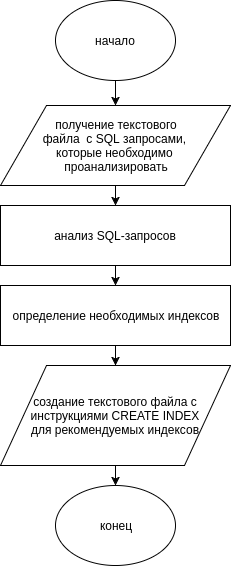
\includegraphics[scale=0.5]{index-advisor-postgresql.png}
  \caption{Процесс работы Index Advisor для PostgreSQL}
  \label{img:index_advisor_postgresql}
\end{figure}

\paragraph{Требования к разрабатываемому инструменту}
\begin{enumerate}
\item Считывание текстового файла с набором SQL запросов. Каждый запрос записывается в одну строку. Несколько запросов разделяется символом ";" и переводом строки;
\item В зависимости от считанного файла, в случае успеха разбора всех запросов, программа должна возвращать 0, а в случае ошибки, хотя бы в одном запросе, ненулевое значение, которое, как правило, интерпретируется, как код ошибки. Если встречается ошибка, то прекратить дальнейший разбор файла;
\item Для успешно считанных индексов создать файл-скрипт с инструкциями CREATE INDEX для создания индексов для этих запросов.
\end{enumerate}

\paragraph{Тестирование разрабатываемого инструмента} 

Правильность работы инструмента необходимо проверить на эксперементальной БД с помощью:
\begin{enumerate}
\item команды \textit{EXPLAIN}, доказывающим, что СУБД использует построенный индекс при выполнении данного запроса;
\item команды \textit{SHOW PROFILER}, доказывающим уменьшение времени выполнения запросов после добавления индекса.
\end{enumerate}
